\documentclass{article}
\usepackage[utf8]{inputenc}
\usepackage{graphicx}

\usepackage[T1]{fontenc}


% set font encoding for PDFLaTeX or XeLaTeX
\usepackage{ifxetex}
\ifxetex
  \usepackage{fontspec}
\else
  \usepackage[T1]{fontenc}
  \usepackage[utf8]{inputenc}
  \usepackage{lmodern}
\fi

% used in maketitle
\title{
Reporte de actividad 1}
\author{José Pablo Montaño De la Ree}
\date{Enero 30,2018}


% Enable SageTeX to run SageMath code right inside this LaTeX file.
% documentation: http://mirrors.ctan.org/macros/latex/contrib/sagetex/sagetexpackage.pdf
% \usepackage{sagetex}

\begin{document}
\maketitle


\section{Introduccion}

La atmosfera terrestre esta conformada por diferentes gases, esta capa que se mantiene cerca de nuestro planeta por la gravedad del mismo, ayuda a propiciar la vida protegiendo al planeta de rayos ultravioleta, reteniendo calor y permitiendo la existencia de agua. Esta es 78.09\% de hidrogeno, 20.95\% de oxigeno, .93\% de argón y .04\% de dioxido de carbono. Aunque no se tiene ubicado de forma exacta el final de la atmosfera, tres cuartas partes de su masa de  $5.5x10^{18}$ kg, estan ubicados en los primeros 11km de la superficie de la tierra al espacio.

\begin{figure}[h!]
  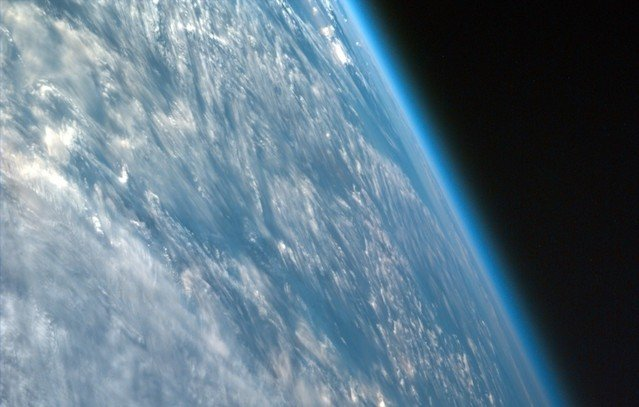
\includegraphics[width=\linewidth]{atmosphere.jpg}
  \caption{Nasa, Septiembre 5 2008,Oblique shot of Earth,https://www.jpl.nasa.gov/spaceimages/details.php?id=PIA11066}
  \end{figure}

\section{Capas de la atmosfera}

La atmosfera, esta compuesta por diferentes capaz, las cuales han sido clasificadas en sus alturas. La más cercana a la tierra es la Troposfera, que se encuentra en los primeros 12km.La cual pierde su temperatura al aumentar la altura, ya que esta recive su calor de la superficie de la tierra, lo cual lleva a una mescla vertical de la temperatura. unida al limite superior de la troposfera esta la tropopausa. que es donde ocurre una invercionn de temperatura.
\linebreak



La segunda capa es la estratosfera, la cual esta comprendida de los 12km a los 50km, terminando en la estratopausa que mide 5km. En esta, entre más aumenta la altura tambien la temperatura, esto es poque esta capa contiene la capa de ozono, la cual absorbe los rayos ultravioleta, haciendo que su teperatura varia de -60 grados centrigrados a 0 grados centrigraods.
\linebreak


La capa conocida como mesosfera, seria la siguiente en orden, que mide 30km desde el final de la capa anteriror, la cual colinda con la mesopausa con un largo de aproximadamnete 5 km.esta capa tienen una temperatura promedio de -85 gracos celcius. 
\linebreak

La siguiente capa es la termosfera la cual se encuentral se encuentradesde la altura de 80 km a la de 700km, junto con la teropausa que se encuentra ente los 500km y los 1000km de latura. Esta capa que tambien contienen a la ionosfera es tan poco densa que no logra transmitir energia. y su temperatura maxima puede ser de 1500 grados celcius. 
\linebreak

Por ultimo seria la exosfera, la cual esta entre los 700km  y los 10,000km, donde esta se encuentra con el viento solar. La densidad es tan baja que las particulas pueden viajar miles de kilometros sin chocar con otras.
\linebreak

\section{Propiedades Fisicas y propiedades opopticas}

La atmosfera tiene ciertas caracteristicas fisicas que valen la pena mencionar.La atmosfera proboca una presion sobre la tierra de 101325 pasacales. La densidad de esta varia de forma esponencial reduciendoce por la mtad cada 5.6 km, por lo cual podemos deducir que no esta distribuida uniformemente.  Al variar la temperatura y la denisdad de la atmosfera de esa forma, la velocidad del sonido tambien varia a lo largo de la atmosfera.
\linebreak
La atmosfera, tambien tiene propiedades opticas interesantes. la dispercion de la luz solar por ejemplo,que provoca que los fotones no llegen directamente.Esta tambien absorbe un rango de la luz que va desde los 300nm a la luz visible. Esta tambien emite en el rango infrarrojo devido a su temperatura. Esta absosorcion y emicion estan directamente relacionadas con el efecto greenhouse. Como ultimo, el inidice de refraccion de la atmosfera es de 1, sin embargo este aumenta con la temperatemperatura, lo cual da origen a los espejismos.

\section{Circulacion}

La circulacion atmosferica es la gran circulacion del aire por la troposfera. Este fenomeno determinado por la rotacion de la tierra varia poco,  y es reponsable de la distribucion de temperatura global.

\section{Referencias}
Wikipedia. (2017). Atmosphere of Earth. 29 de enero del 2018, de Wikipedia Sitio web: https://en.wikipedia.org/wiki/Atmosphere\_of\_Earth\#Physical\_properties

\section{Referente a la actividad}

¿Qué fue lo que más te llamó la atención de esta actividad?
El como las propiedades de la atmosfera cambian de forma no uniforme al igual que la distribucion de esta.  Y en cuanto Latex en como esta construido para facilitar el trabajo de ensayos, sin embargo, es algo complicado y a la vez amigable.
\linebreak

¿Qué fue lo que se te hizo menos interesante?
Que puedo escribir en el docuemnto sin poner comillas como en fortran.
\linebreak

¿Qué cambios harías para mejorar esta actividad? 
Se utilizaria un texto en español.
\linebreak

¿Cuál es tu primera impresión de uso de LATEX?Es muy lento trabajar en Latex
\linebreak
¿El tiempo sugerido para esta actividad fue suficiente? Si
\linebreak
¿Encontraste algún documento o recurso en línea útil que quisieras compartir con los demás?Si
\linebreak
http://www.cva.itesm.mx/biblioteca/pagina\_con\_formato\_version\_oct/apa.htm, te crea referencias APA.





\end{document}
